%subsection
\begin{comment}
IoTサービスの開発と運用における要件を引き出すために、岡本商店街での実験を行った。
・実験の概要
・開発したサービスの説明
・用いた機器や開発したプログラム等の説明
 ・どのように開発したのか
\end{comment}

\subsubsection{実験概要}
2015年12月8日から2016年2月26日まで、NPO法人コミュニティリンクへのインターンシップの一環として、岡本商店街にて人流観測を行った。
岡本商店街とは、神戸市東灘区にある阪急岡本駅とJR摂津本山駅の間にある商店街のことである。
実験は、商店街の方に人流を可視化するIoTサービスを提供し、商店街の活性化に役立てるといった趣旨で行った。
観測は、2016年2月7日から2016年3月14日まで行った。

人流観測とは、各地点から各地点迄をある時に移動した人数を観測するものである。
通常は、観察員がカウンタを用いて数えるが、それでは各地点間を移動した人数はわかるが、その人が以前どの地点に居たのかはわからない。
そこで、携帯電話についているWifi機能を利用し、観測を行うこととした。
携帯電話のWifi機能は、無線LANの接続に使われるが、接続毎にWifi機能を有効にすることが手間なため、常時ONにしている人も少なくない。
携帯電話のWifi機能を有効にしている場合、携帯電話から接続可能な無線LANを探す為、プローブパケットというものが定期的に送出される。
プローブパケットには、そのプローブパケットを送出した機器の物理アドレスが含まれており、個々の機器が識別可能である。
そのプローブパケットを複数地点で観測し、含まれている物理アドレスと受信時刻を照合することで、携帯電話端末を持った人がどのように移動をしたのかが分かる。
岡本商店街では、この原理を利用して、人流観測を行った。

\subsubsection{観測・分析・可視化システムの構成}
岡本商店街の5店舗に開発した観測機器を設置し、サーバにて蓄積・分析・可視化を行った。
構成としては、観測機器内で動作するプログラムが定期的にサーバーに観測データを送信する。
サーバ上では、分析プログラムと可視化プログラムが動作しており、観測データは分析プログラムへ渡される。
分析プログラムは、観測データを可視化プログラムの要求によって分析し、結果を可視化プログラムへ渡す。
可視化プログラムは、ユーザからの操作によって分析プログラムを呼び出し、分析結果をWebインターフェースによって可視化する。
このシステムのユーザーは、ブラウザからWebインターフェースへアクセスすることで、操作・分析結果の閲覧をすることができる。
図\ref{fig:okamoto_diag1}は、開発したシステムの構成を示している。
\begin{figure}[htbp]
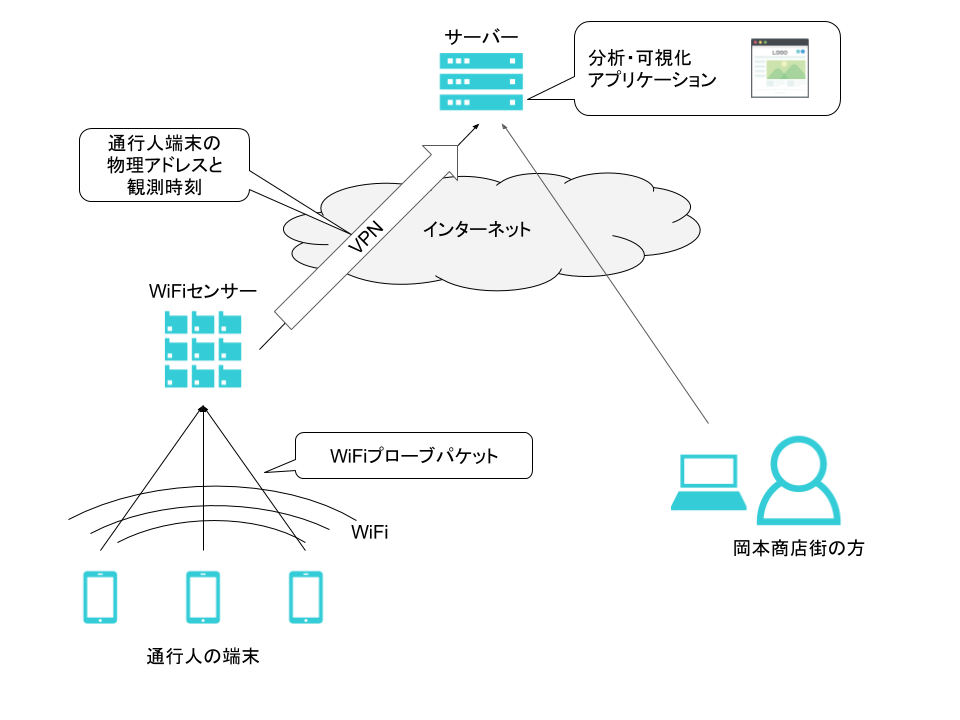
\includegraphics[width=16cm]{images/okamoto_diag1.png}
\caption{岡本商店街人流観測 構成図}
\label{fig:okamoto_diag1}
\end{figure}

開発した観測機器は、RaspberryPiとBaffalo製のWifiドングル、ampsence・rsyncというソフトウェアを利用し作成した。
図\ref{fig:okamoto_pict1}は、開発した観測機器である。
\begin{figure}[htbp]
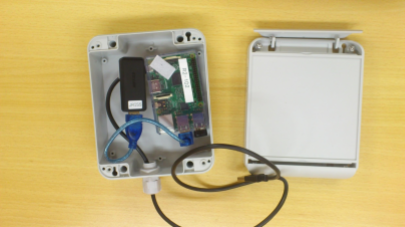
\includegraphics[width=16cm]{images/okamoto_pict1.png}
\caption{岡本商店街人流観測 使用した機器}
\label{fig:okamoto_pict1}
\end{figure}
RaspberryPiとは、小型PCの一つで安価に入手が可能である。
また、利用したRaspberryPiにはWifiインターフェースが存在しなかったので、Baffalo製のUSB接続が可能なWifiドングルを接続した。
ampsenceとは、プローブパケットを受信しプローブパケットに含まれる物理アドレスと観測日時をファイルへ記録するソフトウェアである。
rsyncとは、ディレクトリの中を同期させるプログラムで、遠隔にあるコンピュータの指定したディレクトリの中と、手元のコンピュータの指定したディレクトリを同期することができる。
開発した観測機器は、起動時にampsenceを動作させ、定期的にrsyncを実行するよう設定した。
これによって、各所に設置された観測機器の情報をサーバー上に集約・蓄積する。

作成した分析プログラムは、可視化プログラムから指定された期間内の観測データを読み込み、地点ごと観測時間ごとの物理アドレスの数の推移・地点ごと観測時間ごとの移動した人数の割合を集計し、可視化プログラムへ渡す。
作成した可視化プログラムは、ユーザから指定された期間を分析プログラムへ渡し、分析結果を棒グラフや円グラフといった形で、ユーザーへ表示する。
図\ref{fig:okamoto_ss}は作成したWebアプリケーションである。
\begin{figure}[htbp]
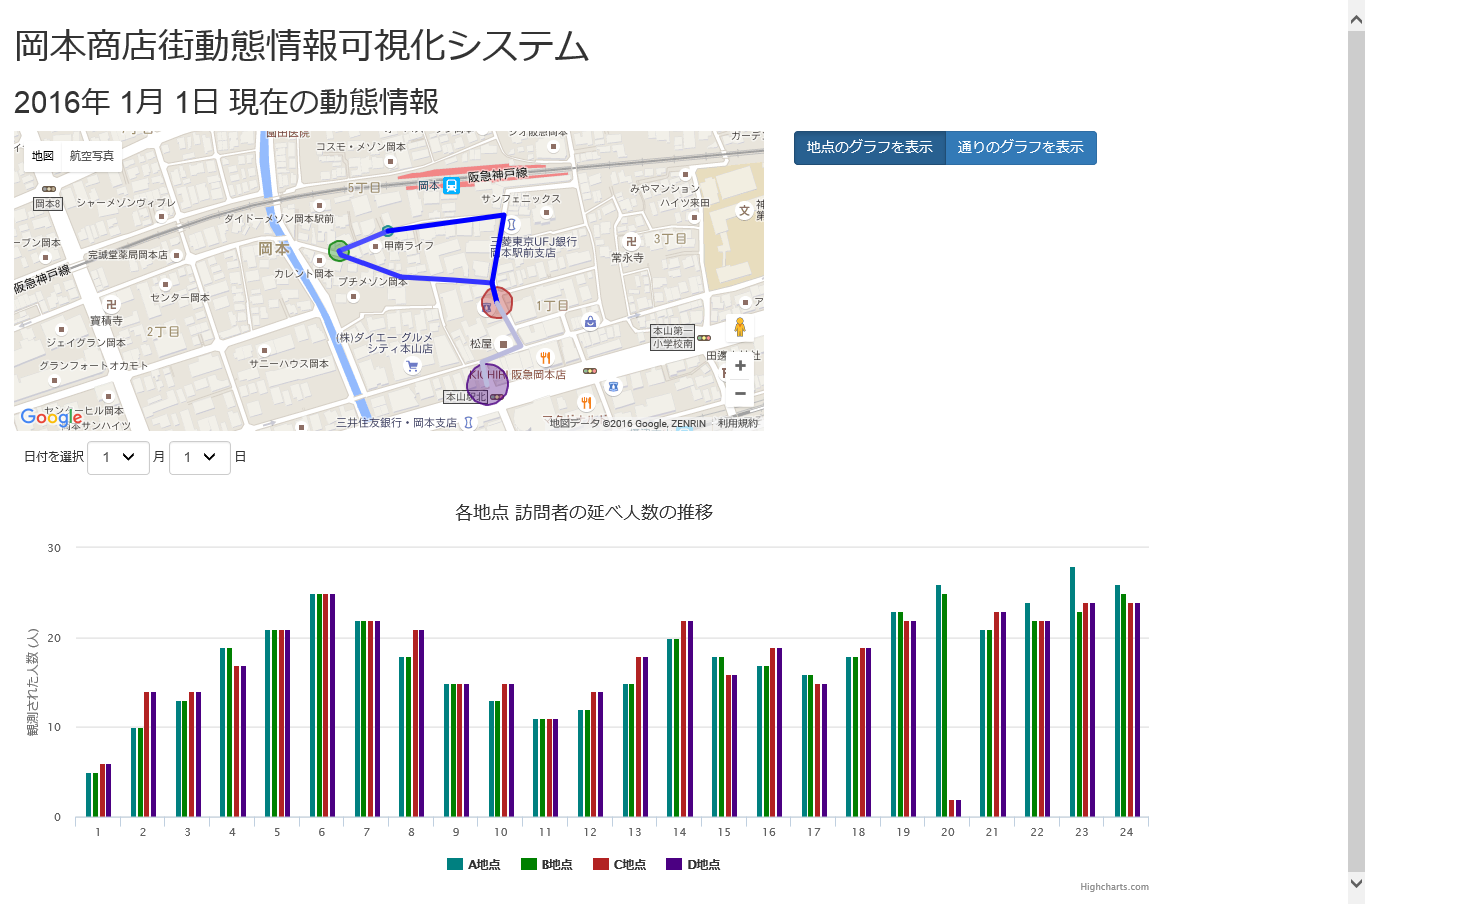
\includegraphics[width=16cm]{images/okamoto_scr1.png}
\caption{岡本商店街人流観測可視化アプリケーションスクリーンショット}
\label{fig:okamoto_ss}
\end{figure}

観測機器からサーバまでのネットワークは、観測した物理アドレスが流れるという点、ソフトウェアのアップデートの為にログイン可能にしたいといった要望から、VPNを使用した。
VPNには、OpenVPNを使用した。

また。観測機器、分析・可視化アプリケーションを開発するにあたって、次のような点を考慮した。
\begin{itemize}
\item ネットワーク機器の設定が不要であること\\
	機器が設置されるネットワークは、店舗のネットワークである。
	そのため、ネットワーク機器の設定を変更することはできない。
	よって、観測機器と分析・可視化アプリケーションの連携が、ネットワーク機器の設定に左右されないよう設計する必要があった。
\item トラブル対応のしやすさ\\
	機器が設置される場所は、岡本商店街内の店舗である。
	そのため、設置やトラブル対応、回収については、予め店舗に連絡を入れなくてはならない。
	また、夜間や店舗の休日に対応することは困難である為、遠隔から観測機器にログインする必要があった。
\item 設置箇所の問題\\
	店舗によっては、店舗内に無線ネットワークが存在しなかったので、後術するSORACOM Airを用いることとした。
\item データ損失に備える\\
	サーバー側の不良によって観測データが損失する事に備え、機器自体にも情報を蓄積しておくことにした。
\end{itemize}

\subsubsection{考察}
%開発者が構造の複雑さ、運用者が利便性のなさから来る問題を抱えている。

しかし、実験には次のような困難があった。
\begin{itemize}
\item ネットワークの設定に手間取った。
\item 設定ミスがあった。
\item 電源が抜けていたことがあった。
\item 一つのトラブルに対し、現地に何度も行かなくてはならなかった
\item 長時間に渡って観測データが欠損していることがあった。
\end{itemize}

これら困難から、このような問題があることが分かった。
\begin{itemize}
\item トラブルに気づくのが遅れた問題\\
	トラブルが発生していても、誰も気づかなかった事があった。
	そのため、トラブルへの対応が遅れ、観測できなかった事があった。
\item トラブル対応が困難な問題\\
	ネットワークによる問題なのか、電源が抜けているといった問題なのか、切り分けが難しく、
	トラブルがあった際に、開発者が対応しなければならないのか運用者で良いのか判断がつきにくかった。
	そのため、開発者が行っても、電源が抜けているだけの問題であったり、運用者が行っても解決できない為、再度現地に行く事になることがあった。
	また、トラブルの対応を検討している間に、機器の再起動等により復旧してしまった事もあった。
\item 観測データの欠損から、満足な分析ができなかった問題\\
	トラブルと、トラブルへの対応の遅れから、観測データが足りず、満足な分析が行えなかった。
	また、観測できていなかった日時を推測するため、観測データを何度も参照する事になり、分析に手間取った。
\end{itemize}

これらから、次のような機能を持つ監視が必要であることが分かった。
\begin{itemize}
\item トラブル発生時に、ネットワークの問題なのかそれ以外の問題なのか、ある程度切り分けることができること。
\item トラブルのあった日時が記録されている必要があること
\item 現在の機器の状態を簡単に閲覧できる必要があること。
\end{itemize}


